
%%%%%%%%%%%%%%%%%%%%%%%%%%%%%%%%%%%%%%%%%%%%%%%%%%%%%%%%%%%%%%%%%%%%%%%%%
%           Capítulo 2: MARCO TEÓRICO - REVISIÓN DE LITERATURA
%%%%%%%%%%%%%%%%%%%%%%%%%%%%%%%%%%%%%%%%%%%%%%%%%%%%%%%%%%%%%%%%%%%%%%%%%

\chapter{Marco teórico}

\section{Articulaciónes y grados de libertad}

La movilidad de un sistema puede expresarse en función de los parámetros independientes mínimos que se necesitan para describir de manera única su posición y orientación en un instante de tiempo (Norton, 2009). Estos parámetros reciben por \textbf{nombre grados de libertad} (GDL). El número de GDL también depende de las dimensiones del espacio en el que se trabaje. Para ejemplificar el caso del movimiento en un espacio plano de dos dimensiones se puede tomar un cuadrado de papel y colocarlo sobre un escritorio, el papel puede moverse de manera vertical (primer GDL), horizontal (segundo GDL) o girar (tercer GDL). Dichos movimientos también pueden limitarse. Si ahora se toma un alfiler y se clava el cuadrado de papel sobre el escritorio se han restringido los movimientos horizontales y verticales, quedando únicamente la rotación alrededor del alfiler (solamente un GDL).
\\

En el caso del movimiento plano, los cuerpos rígidos sin restricción cuentan con tres
GDL, dos que indican posición y uno que indica orientación. Si se considera ahora el
espacio tridimensional, los cuerpos rígidos cuentan con seis GDL, se necesitan tres para
definir la posición y otros tres que definen la orientación. Se ilustran estos ejemplos en
la figura (\ref{figGDL}).

\begin{figure}
	\centering
	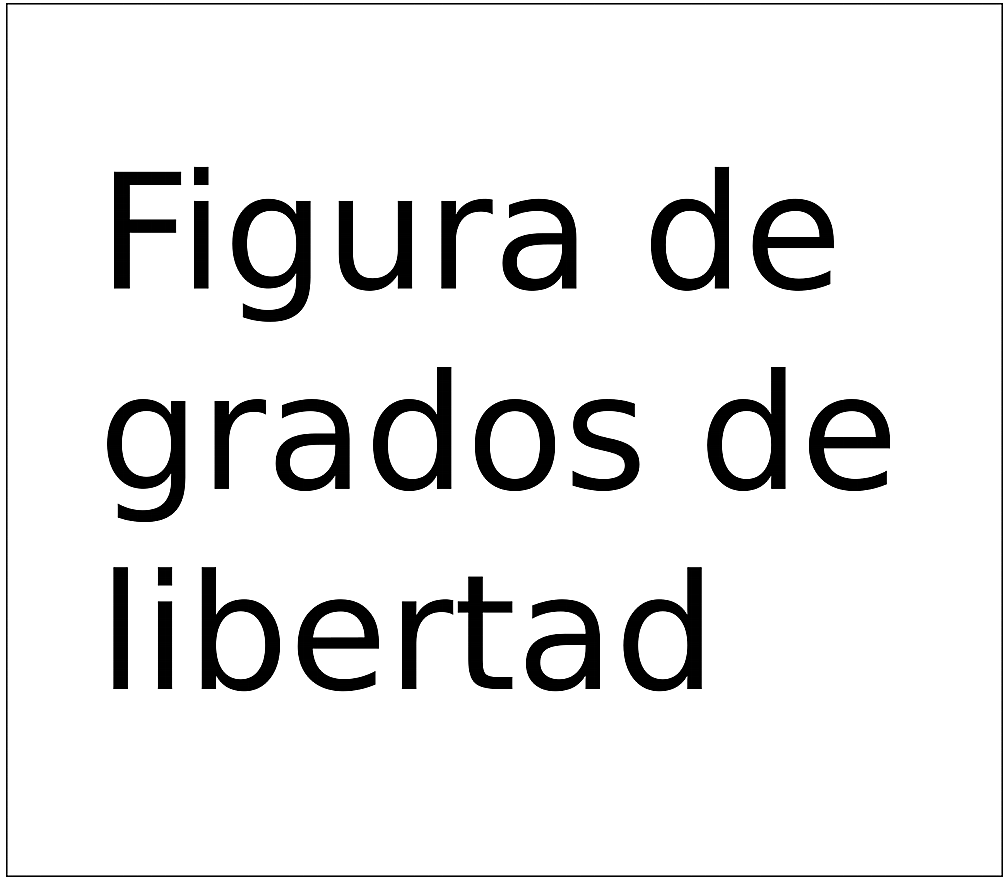
\includegraphics[scale=0.1]{Capitulo2/figs/GDLs.png}      %Ruta completa de la imagen, porque se compila desde el archivo tesis.tex
	\caption{Grados de libertad en movimiento plano y en movimiento tridimensional}            %Pie de imagen
	\label{figGDL}                            %nombre de referencia
\end{figure}

Los eslabones que componen a un robot manipulador están conectados de tal manera
que se permita cierto tipo de movimiento. Existen dos movimientos a partir de los cuales se derivan cualquier movimiento complejo conocido: la traslación pura y la rotación
pura.
Estas conexiones entre eslabones reciben el nombre de articulaciones o pares cinemáticos.

\begin{figure}[!h]
	\centering
	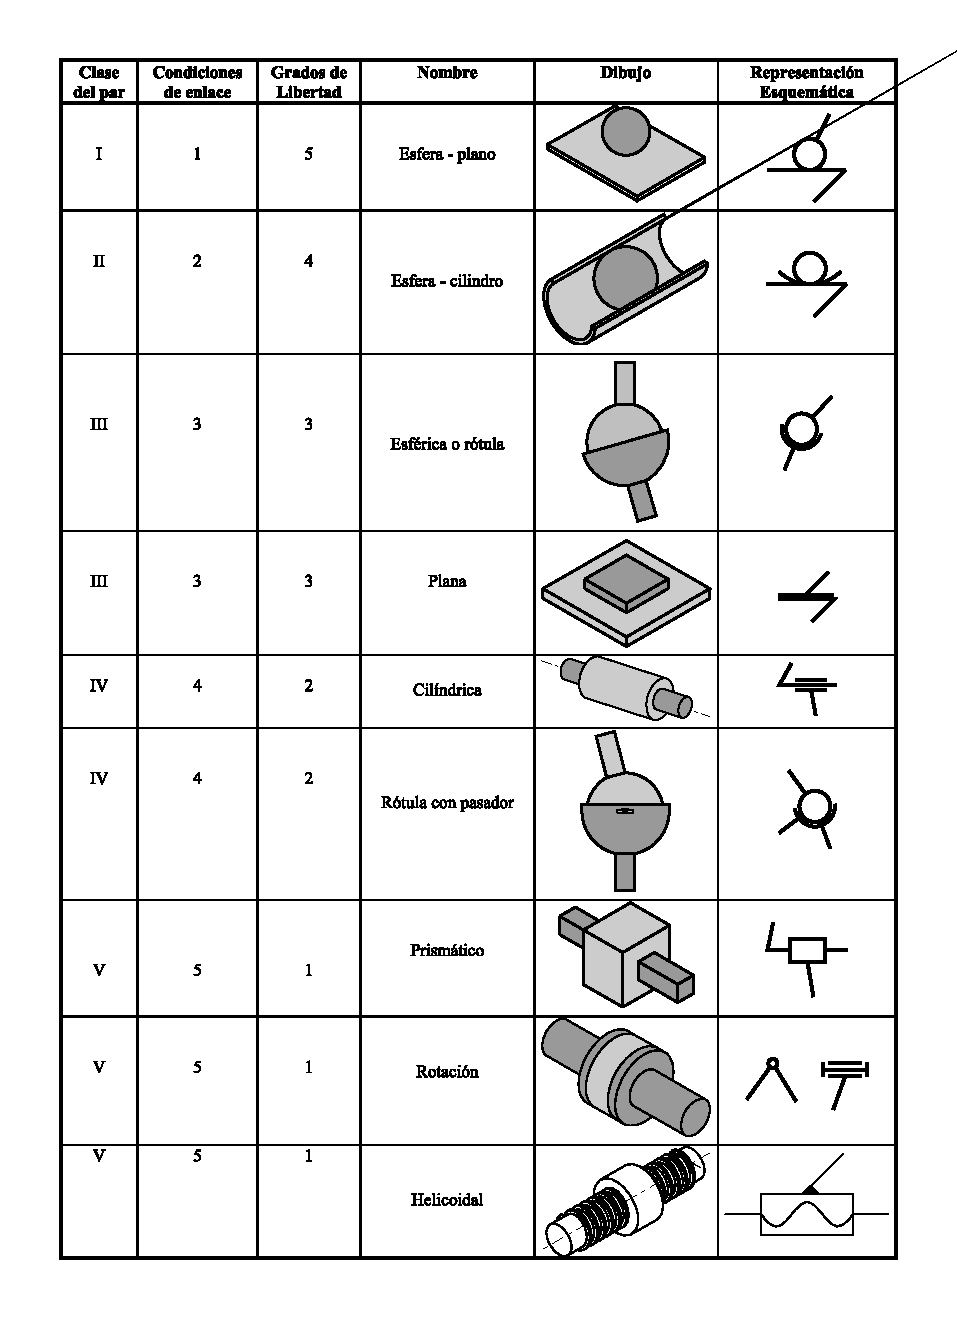
\includegraphics[scale=0.8]{Capitulo2/figs/Pares.pdf}      %Ruta completa de la imagen, porque se compila desde el archivo tesis.tex
	\caption{Tipos de pares cinemáticos y su representación}            %Pie de imagen
	\label{figPares}                            %nombre de referencia
\end{figure}

\section{Cinemática del manipulador}
